\section{Introduction}
\label{sec:introduction}


\par The objective of this laboratory assignment was to create a circuit that would transform an input AC voltage of amplitude 230V and frequency of 50 Hz to an output DC voltage of amplitude 12V and frequency 50Hz. To do this, an Envelope Detector, a Voltage Regulator and a Transformer were used. This last component was not actually modeled in the simulation and theoretical analysis. It was considerared that the transformer would be represented with an alternated, independent voltage source that would connect to the envelope detector and would reduce the input amplitude of 230V by a ratio of n:1. This ratio will be decided during the simulation and theorethical analysis. Do note that n can be any rational number, as a large number of coils are used in any real transformer, thus allowing for a great deal of freedom in choosing the transformer ratio.\par
To determine the quality of the circuit, when compared to others, a merit classification system was created. This merit system took into account the cost of the components used, as well as the ripple and average amplitude of the output voltage. The merit of the circuit will determined according to the following equation: 
\begin {equation}
	 MERIT = \frac{1}{cost*(ripple_{reg} + |average_{reg} - 12| + 10^{-6})}   	
	\label{eq:i1}
\end{equation}

and the cost of the componets are the following: cost of resistors = 1 monetary unit (MU) per kOhm, cost of capacitors = 1 MU/uF
and cost of diodes = 0.1 MU per diode. The voltage source that represents the transformer was not taken into account in the cost, and so the parameter n was regarded as a "free" parameter.
 
The general layout of the circuit that was implemented can be seen in \textbf{Figure~\ref{fig:circuit_t3}}. In the next sections the actual architecture implemented will be analyzed in greater detail.\par
\begin{figure}[h] \centering
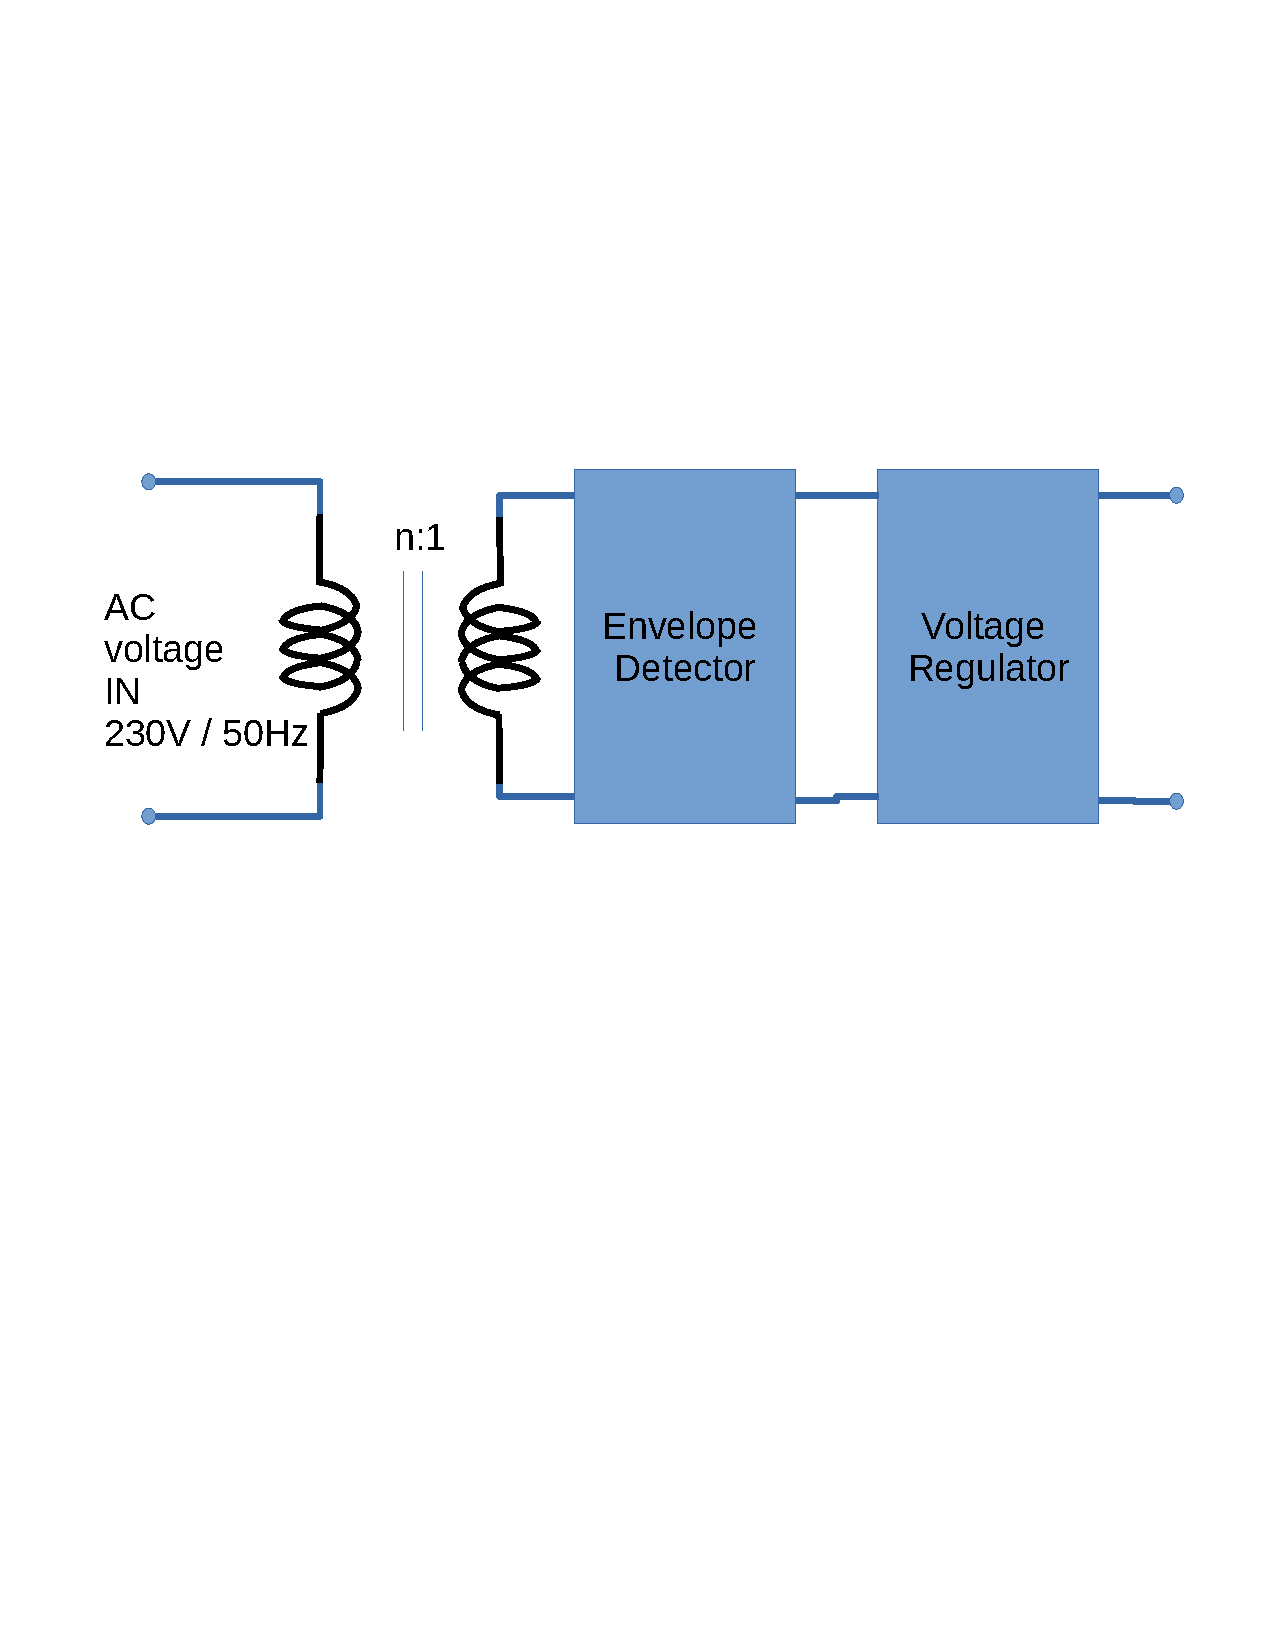
\includegraphics[width=0.6\linewidth]{circuit_t3.pdf}
\vspace{-6cm}
\caption{Circuit in study}
\label{fig:circuit_t3}
\end{figure}


In Section~\ref{sec:analysis}, a theoretical analysis of the circuit is
presented. Here the circuit is analised using suitable theoretical models for the diodes, in order to predict the output of the Envelope Detector
and Voltage Regulator circuits. The output DC level and the
voltage ripple are calculated and the plots for the voltages at the output of the Envelope Detector and Voltage Regulator circuits are presented, as well as the plot for the output deviation (output voltage subtracted by a factor of 12), of the output of the regulator. 
In Section~\ref{sec:simulation}, the circuit is analysed by
simulation using the program Ngspice. In Ngspice the default model for the diode was used. The AC/DC converter was simulated for 10 periods and the voltage average and ripple were measured using built in functions of the program. The same plots produced in the theoretical analysis were made in this section, here by simulation. The conclusions of this study are outlined in
Section~\ref{sec:conclusion}, where the theoretical results obtained in
Section~\ref{sec:analysis} are compared to the simulation results obtained in
Section~\ref{sec:simulation}.





\pagebreak

